\documentclass[9pt]{beamer}
\usepackage{kotex}
\usepackage{amsfonts,amssymb,amsthm}
\usepackage[dvipsnames]{xcolor}
\usepackage{xcolor}
\usepackage{etoolbox}
\usepackage{braket}
%## color
\definecolor{customBlack}{HTML}{3B4252}
\definecolor{customBlackGrey}{HTML}{434C5e}
\definecolor{cuatomGrey}{HTML}{4C566A} 
\definecolor{customWhite}{HTML}{ECEFF4} 
\definecolor{customBlue}{HTML}{6082B6}  
\definecolor{customRed}{HTML}{BF616A}
\definecolor{vividauburn}{rgb}{0.58, 0.15, 0.14}


%## Theme & custom
% \usetheme{metropolis}           % Use metropolis theme
% \metroset{block=fill}
\usetheme{moloch} % modern fork of the metropolis theme
\molochset{block=fill}
\setbeamersize{text margin left=5mm, text margin right=5mm}
\setbeamercolor{palette primary}{bg=customBlack}
\setbeamercolor{alerted text}{fg=customRed}
\setbeamercolor{itemize item}{fg=customBlue}


%## font
\usefonttheme[onlymath]{serif}
% \setbeamerfont{normal text}{size=\small}
% \setbeamerfont{math text}{size=\tiny}


%## Theorem title, numbering
\makeatletter
\setbeamertemplate{theorem begin}
{%
\begin{\inserttheoremblockenv}
{%
\inserttheoremheadfont
\inserttheoremname
\ifx\inserttheoremaddition\@empty\else\ of\ \inserttheoremaddition\fi%
\inserttheorempunctuation
}%
}
\setbeamertemplate{theorem end}{\end{\inserttheoremblockenv}}
\makeatother
\setbeamertemplate{theorems}[numbered]  


%## Custom block
\setbeamercolor{block title}{bg=customBlue, fg=white}
\setbeamercolor{block body}{bg=customWhite, fg=customBlack}
\setbeamercolor{block title alerted}{%
    use={block title, alerted text},
    bg=customRed,
    fg=white
}
\setbeamercolor{block body alerted}{%
    use={block title, alerted text},
    bg=customWhite,
    fg=customBlack
}
\AtBeginEnvironment{definition}{%
    \setbeamercolor{block title}{fg=white,bg=customBlackGrey}
    \setbeamercolor{block body}{fg=customBlack, bg=customWhite}
}
\AtBeginEnvironment{theorem}{%
    \setbeamercolor{block title}{fg=white,bg=customBlackGrey}
    \setbeamercolor{block body}{fg=customBlack, bg=customWhite}
}
\AtBeginEnvironment{corollary}{%
    \setbeamercolor{block title}{fg=white,bg=customBlackGrey}
    \setbeamercolor{block body}{fg=customBlack, bg=customWhite}
}
\AtBeginEnvironment{lemma}{%
    \setbeamercolor{block title}{fg=white,bg=customBlackGrey}
    \setbeamercolor{block body}{fg=customBlack, bg=customWhite}
}

\title{1. Review of Probability}
\date{\today}
\author{Vaughan Sohn}
% \institute{Centre for Modern Beamer Themes}


\begin{document}
    %#################################### 
    \maketitle
    
    %#################################### 
    \begin{frame}
        \frametitle{Contents}
        \tableofcontents
    \end{frame}

    \begin{section}{Learn from Example: Card game}
      \begin{frame}{Example}
        \begin{itemize}
          \item 다음과 같은 3종류의 카드가 존재한다고 가정하자.
          \begin{itemize}
            \item Red / Red
            \item Red / Black
            \item Black / Black
          \end{itemize}
          \item 눈을 감고 하나의 카드를 고른 뒤, 그 카드의 한쪽 면을 확인한다.
          \item Question: 내가 고른 카드의 한쪽 면의 색상이 "Red"일 때, 다른 면의 색상도 "Red"일 확률은 얼마인가?
        \end{itemize}
        \vspace{1cm}
        
        \begin{alertblock}{Prior knowledge}
        \checkmark 이 문제를 풀기 위해서는 "Conditional probability"의 개념에 대해서 이해해야한다. 지금부터 하나하나 확률의 개념들에 대해서 복습하면서 이 예제 문제를 풀어보도록 하자.
        \end{alertblock}
      \end{frame}
    \end{section}

    \begin{section}{Random variable and Probability distribution}
      \begin{frame}{Random variable}
        \begin{definition}[random variable]
          A \textbf{random variable} is a real-valued \textit{function} of the outcome of the experiment.
          $$X: \Omega \rightarrow \mathbb R$$
        \end{definition}
        \begin{definition}[sample space, atom]
            A \textbf{sample space} $\Omega$ is a set of all possible outcomes, and the elements of that set are called \textbf{atoms}.
        \end{definition}
        \checkmark \underline{meaning}: Random variable은 \textit{numerical value가 아닐 수도 있는} 실험 결과(e.g., 동전 앞면이 나왔다.) 를 numerical value로 할당해준다. 
        \begin{itemize}
          \item Outcome은 어떠한 \alert{확률}에 의하여 그 값이 결정되는 실험의 결과를 의미한다.  
          \item Random variable과 sample space 그리고 atom간의 관계는 다음과 같다.
          
          \vspace{0.3cm}

          \begin{figure}
            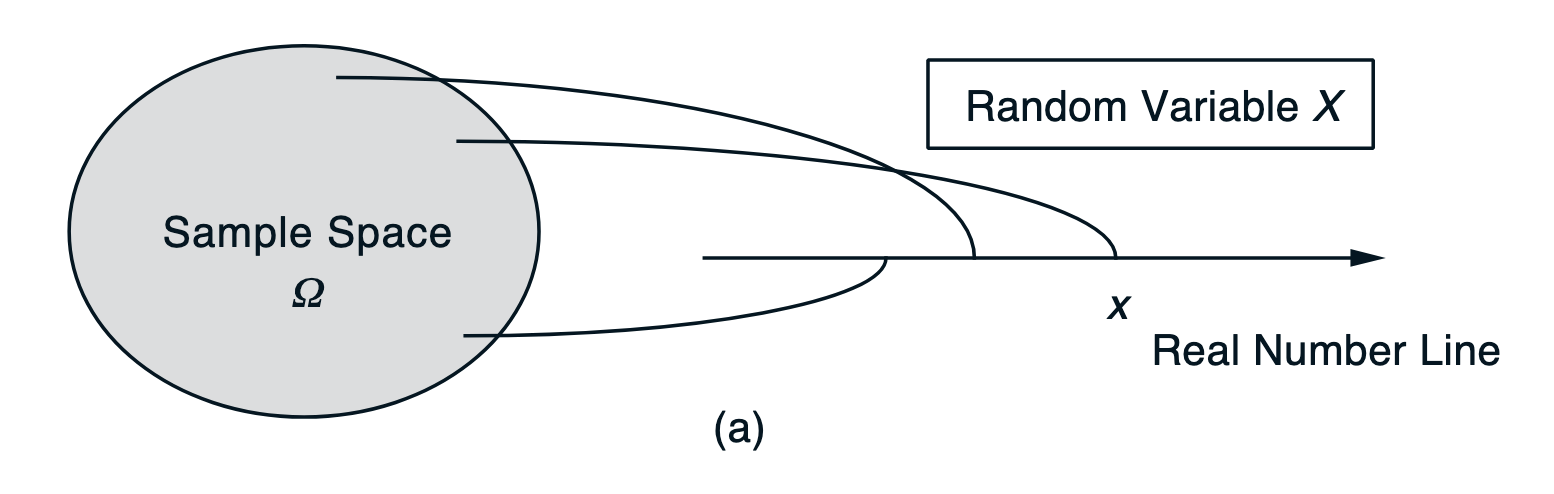
\includegraphics[width=0.5\columnwidth]{image/L1-sample_space.png}
            \end{figure}
        \end{itemize}
      \end{frame}

      \begin{frame}{Discrete probability distribution}
        \begin{definition}[probability law]
          \textbf{Probability distribution} assigns to a set $A$ of possible outcomes a \textit{nonnegative} number $P(A)$. 
        \end{definition}
        \checkmark \underline{meaning}: Random variable이 실험 결과를 numerical value로 할당하는 것처럼, probability distribution은 numerical value를 $(0, 1)$사이의 양의 실수값으로 매핑해준다.
        $$P: X \rightarrow [0,1]$$
        \begin{itemize}
          \item 전체 sample space에 대한 확률 분포의 합은 1이 되어야한다. 
          $$\sum_{x \in \mathcal X} P(X=x) = 1$$
          \item If sample space is finite, we call a probability law as \textbf{discrete probability distribution}.
        \end{itemize}
      \end{frame}

      \begin{frame}{Expectation and Variance}
        \begin{definition}[expectation]
          An \textbf{expectation} of random variable $X$ is 
          $$ \mathbb E [X] = \sum_{x \in \mathcal X} x \cdot P_X(x).$$
        \end{definition}
        \begin{definition}[variance and standard deviation]
          An \textbf{variance} of random variable $X$ is 
          $$ \operatorname{Var}(X) = \mathbb E[(X - \mathbb E[X])^2].$$
          And we called the square root of the variance as \textbf{standard deviation} of $X$.
          $$ \sigma_X = \sqrt{\operatorname{Var}(X) } $$
        \end{definition}
        \begin{itemize}
          \item $X$의 variance는 항상 nonnegative이다.
          \item Variance는 실제 outcome들이 expectation을 기준으로 얼마나 산재되어있는지를 나타내는 척도이다.
        \end{itemize}
      \end{frame}

      \begin{frame}{Probability of the event}
        \begin{definition}[event]
          \textbf{Event} is only a \alert{subset of atoms}.
        \end{definition}
        \begin{theorem}[probability of the event]
          For any event $E$, we have 
          $$P(X\in E) = \sum_{x \in E} P_X(x).$$
        \end{theorem}
        \checkmark \underline{meaning:} Event는 어떤 특수한 조건을 만족시키는 atom들의 집합일 뿐이다. 
        \begin{itemize}
          \item 가능한 모든 event들의 집합을 $\mathcal F$라고 하면, $|\mathcal F|$는 $2^{|\Omega|}$이다.
          \item Example: r.v.가 $D \in \{1, 2, 3, 4, 5, 6\}$ 일 때, 주사위를 던졌을 때 그 결과가 3보다 큰 event의 확률은?
          $$ P(D>3) = \qquad \qquad \qquad \qquad \qquad \qquad \qquad \qquad \qquad  $$
        \end{itemize}
      \end{frame}

      \begin{frame}{Union bound}
        \begin{theorem}[union bound]
          \vspace{-0.5cm}
          \begin{align*} P(E_1 \cup E_2) &= P(E_1) + P(E_2) - P(E_1 \cap E_2)  \\ &= P(E_1 \cap E_2^c) + P(E_1\cap E_2) + P(E_2 \cap E_1^c) \\ &\le P(E_1) + P(E_2)\end{align*}
        \end{theorem}
        \begin{itemize}
          \item Event를 sample space에 있는 집합으로 생각해면 쉽게 이해할 수 있다.
          \\ $\Rightarrow$
          \vspace{1.5cm}
          \item application: 실제로 계산하기 어려운 $P(E_1 \cup E_2)$ 대신 $P(E_1) + P(E_2)$가 0으로 수렴함을 보여서 좌변도 0으로 수렴함을 증명하는 방식으로 활용한다.
        \end{itemize}
      \end{frame}

      \begin{frame}{Joint distribution}
        Let $X$ and $Y$ be random variables associated with the \textit{same experiment}, then the sample space of experiment is $\mathcal X \times \mathcal Y$.
        \begin{definition}[joint distribution]
        The \textbf{joint probability distribution} of $X$ and $Y$ is defined by 
        $$P_{X, Y}(x,y) = P(X=x, Y=y).$$
        \end{definition}
        \begin{definition}[marginalization]
        The \textbf{marginal probability distribution} of $X$ and $Y$ can be obtained from the joint probability distribution,
        $$ P_X(x) = \sum_{y \in \mathcal Y} P_{X, Y}(x, y),\quad  P_y(y) = \sum_{x \in \mathcal X} P_{X, Y}(x, y)$$
        \end{definition}
      \end{frame}

      \begin{frame}{Conditional distribution}
        Let $X$ and $Y$ be random variables associated with the \textit{same experiment}, and we consider a probability distribution when given some \alert{condition}.
        \begin{definition}[conditional distribution]
          The \textbf{conditional probability distribution} of $X$ \alert{given event} $E; Y=y$ is defined by 
          $$P_{X|Y}(x|y) = P(X=x| Y=y)$$
        \end{definition}
        \begin{theorem}
          The conditional PMF[$\ast$] of $X$ given $Y = y$ is related to the joint PMF by
          $$P_{X|Y}(x|y) = \frac{P_{X,Y}(x,y)}{P_Y(y)}$$
        \end{theorem}
      \end{frame}
      \begin{frame}{Conditional distribution}
        \checkmark \underline{meaning:} conditional probability는 given event \alert{set} 안에서 각 outcome의 확률을 나타낸다고 생각하면 이해하기 쉽다. \\ $\Rightarrow$
        \vspace{2cm}
        \begin{itemize}
          \item 현재 우리가 관심있는 r.v. $X$ (i.e., $|$ 왼쪽에 위치한 변수)에 대한 conditional PMF의 합은 1이다. 즉, 여전히 확률로서 동작한다.
          $$\sum_{x \in \mathcal X} P_{X|Y}(x|y) = 1$$
          \item 그러나 r.v. $Y$에 대해서는 그 합이 반드시 1이 되지는 않는다. 
          $$\sum_{y \in \mathcal Y} P_{X|Y}(x|y) \ne 1 \text{ at least, not necessarily.}$$
        \end{itemize}
      \end{frame}
      \begin{frame}{Return to Example}
        \begin{block}{Example}
        \begin{itemize}
          \item 다음과 같은 3종류의 카드가 존재한다고 가정하자.
          \begin{itemize}
            \item Red / Red
            \item Red / Black
            \item Black / Black
          \end{itemize}
          \item 눈을 감고 하나의 카드를 고른 뒤, 그 카드의 한쪽 면을 확인한다.
          \item Question: 내가 고른 카드의 한쪽 면의 색상이 "Red"일 때, 다른 면의 색상도 "Red"일 확률은 얼마인가?
        \end{itemize}
        \end{block}
        \vspace{0.2cm}
        Solution: 
        \vspace{0.1cm}
        \begin{itemize} 
          \item 다음과 같이 2개의 r.v.를 정의하자.
          \begin{itemize}
            \item 첫번째로 확인한 카드의 색상: $X_1 \in \{R, B\}$
            \item 카드의 반대쪽 면의 색상: $X_2 \in \{R, B\}$
          \end{itemize}
          \item 그렇다면, 눈을 감고 고른 카드의 색상을 확인하는 실험결과가 "Red"라는 것을 알고있기 때문에 $X_1 = R$임을 알 수 있다.
          \item 즉, 우리는 다음의 확률을 계산하면 된다.
          $$ P_{X_2|X_1} (R|R) = \frac{P_{X_1, X_2}(R, R)}{P_{X_1}(R)} = \qquad \qquad \qquad  \qquad \qquad \qquad .$$
        \end{itemize}

      \end{frame}
    \end{section}
    \begin{section}{Chain rule}
      \begin{frame}{Chain rule}
        \begin{theorem}[chain rule]
          By definition of conditional PMF, we can write joint PMF as
          \begin{align*} P_{X,Y}(x, y)&=P_{X, Y}(x, y) \frac{P_Y(y)}{P_Y(y)}=P_{X|Y}(x|y) P_Y(y)\\ &= P_{X,Y}(x,y) \frac{P_X(x)}{P_X(x)} = P_{Y|X}(y|x) P_X(x) \end{align*}
          In general, for any set of $N$ variables
          $$ P\left(x_1, \ldots, x_N\right)=\prod_{n=1}^N P\left(x_n | x_1, \ldots, x_{n-1}\right).$$
        \end{theorem}
      \end{frame}
      \begin{frame}{Marginalization}
        \begin{theorem}[marginalization]
          By chain rule, we can get probability distribution on some r.v. from joint PMF as
          $$P_X(x) = \sum_{y \in \mathcal Y} \sum_{z \in \mathcal Z} P_{X, Y, Z}(x, y, z)$$
        \end{theorem}
        $\ast$ \underline{Proof}:
      \end{frame}
    \end{section}

    \begin{section}{Bayes rule}
      \begin{frame}{Bayes rule}
        \begin{theorem}[Bayes rule]
          From the chain rule and marginalization, we get bayes rule
          $$ P(x|y)=\frac{{P}(y|x) {P}(x)}{\sum_x {P}(y | x) {P}(x)} $$ 
        \end{theorem}
        \checkmark \underline{meaning}: 사전확률 $P(y|x), P(x)$로부터 사후확률을 추정할 수 있다. \\
        \vspace{0.4cm}
        applications:
        \begin{itemize}
          \item Let $Y$ be a symptom, $X$ be a disease and interpret the Bayes rule.
          \item Let $Y$ data and $X$ what we want to infer from the data.
        \end{itemize}
        \vspace{2cm}
      \end{frame}
    \end{section}

    \begin{section}{Independence}
      \begin{frame}{Independence}
        \begin{definition}[independence]
          Random variables $X$ and $Y$ are \textbf{independent} $X \perp Y$ if know about the value of $X$(i.e., conditioning event ($X=x$) tell us \textit{nothing} about $Y$. 
          $$ P_{Y|X}(y|x) = P_Y(y)$$ 
        \end{definition}
        \begin{definition}[conditionally independence]
          Random variables $X$ and $Y$ are \textbf{conditionally independent} if know about the value of $X$ tell us \textit{nothing} about $Y$ \alert{given} $Z$. 
          $$ P_{Y|X, Z}(y|x, z) = P_{Y|Z}(y|z)$$ 
        \end{definition}
        \begin{itemize}
          \item 만약 두 r.v.가 independence라면, joint PMF를 인수분해 할 수 있다. [$\ast$]
          $$ P_{X,Y}(x,y) = P_X(x) P_Y(y)$$
          \item 만약 두 r.v.가 conditionally independence라면, joint PMF를 인수분해 할 수 있다.
          $$ P_{X, Y|Z}(x,y|z) = P_{X|Z}(x|z) P_{Y|Z}(y|z)$$
        \end{itemize}
      \end{frame}
      \begin{frame}{Example of Independence and Conditionally Independence}
        \begin{block}{Example}
          \begin{itemize}
            \item 2개의 코인 $C_1$, $C_2$가 있을 때, 각 코인에 대한 PMF가 다음과 같다. 
            \begin{itemize}
              \item $P_{C_1}(H) = 0.5, \quad P_{C_1}(T) = 0.5$
              \item $P_{C_2}(H) = 0.7, \quad P_{C_2}(T) = 0.3$
            \end{itemize}
            \item 즉, $C_1$은 fair coin이고 $C_2$는 앞면의 확률이 더 높은 unfair coin이다.
            \item 두 coin중에서 어떤 coin을 사용할 것인지를 랜덤하게 결정하기 위한 랜덤변수 $Z \in \{1, 2\}$를 가정하자. ($Z \sim U$)
            \item $Z$의 value에 의해 결정된 coin을 2번 flip하고 첫번째 결과에 대한 랜덤변수 $X$, 두번째 결과에 대한 랜덤변수 $Y$를 정의하자.
            \item Question 1: $X \perp Y$?
            \item Question 2: $X \perp Y$, given $Z$?
          \end{itemize}
          \end{block}
          \vspace{0.2cm}
          
          Solution: 
          \vspace{0.8cm}

      \end{frame}
    \end{section}
    \begin{frame}{Appendix}
      \begin{block}{Notations}
        \begin{itemize}
          \item sample space: $\Omega$
          \item random variable: $X, Y, Z, \cdots$
          \item numerical value: $x, y, z, \cdots$
          \item probability for arbitrary outcome: $P(X=x)  = P_X(x)$
          \item expectation of random variable $X$: $\mathbb E[X]$
        \end{itemize}
      \end{block}
    \end{frame}

    \begin{frame}{References}
      \begin{itemize}
        \item D. Bertsekas and J. Tsitsikilis, Introduction to Probability
        \item Lecture notes for EE623: Information Theory (Fall 2024)
    \end{itemize}
    \vspace{6cm}
    \end{frame}
\end{document}